%\VignetteIndexEntry{aheatmap: a Powerful Annotated Heatmap Engine}
%\VignetteDepends{utils,NMF,RColorBrewer,knitr,bibtex}
%\VignetteKeyword{aplot}
%\VignetteCompiler{knitr}
%\VignetteEngine{knitr::knitr}

\documentclass[a4paper]{article}\usepackage[]{graphicx}\usepackage[]{color}
%% maxwidth is the original width if it is less than linewidth
%% otherwise use linewidth (to make sure the graphics do not exceed the margin)
\makeatletter
\def\maxwidth{ %
  \ifdim\Gin@nat@width>\linewidth
    \linewidth
  \else
    \Gin@nat@width
  \fi
}
\makeatother

\definecolor{fgcolor}{rgb}{0.345, 0.345, 0.345}
\newcommand{\hlnum}[1]{\textcolor[rgb]{0.686,0.059,0.569}{#1}}%
\newcommand{\hlstr}[1]{\textcolor[rgb]{0.192,0.494,0.8}{#1}}%
\newcommand{\hlcom}[1]{\textcolor[rgb]{0.678,0.584,0.686}{\textit{#1}}}%
\newcommand{\hlopt}[1]{\textcolor[rgb]{0,0,0}{#1}}%
\newcommand{\hlstd}[1]{\textcolor[rgb]{0.345,0.345,0.345}{#1}}%
\newcommand{\hlkwa}[1]{\textcolor[rgb]{0.161,0.373,0.58}{\textbf{#1}}}%
\newcommand{\hlkwb}[1]{\textcolor[rgb]{0.69,0.353,0.396}{#1}}%
\newcommand{\hlkwc}[1]{\textcolor[rgb]{0.333,0.667,0.333}{#1}}%
\newcommand{\hlkwd}[1]{\textcolor[rgb]{0.737,0.353,0.396}{\textbf{#1}}}%

\usepackage{framed}
\makeatletter
\newenvironment{kframe}{%
 \def\at@end@of@kframe{}%
 \ifinner\ifhmode%
  \def\at@end@of@kframe{\end{minipage}}%
  \begin{minipage}{\columnwidth}%
 \fi\fi%
 \def\FrameCommand##1{\hskip\@totalleftmargin \hskip-\fboxsep
 \colorbox{shadecolor}{##1}\hskip-\fboxsep
     % There is no \\@totalrightmargin, so:
     \hskip-\linewidth \hskip-\@totalleftmargin \hskip\columnwidth}%
 \MakeFramed {\advance\hsize-\width
   \@totalleftmargin\z@ \linewidth\hsize
   \@setminipage}}%
 {\par\unskip\endMakeFramed%
 \at@end@of@kframe}
\makeatother

\definecolor{shadecolor}{rgb}{.97, .97, .97}
\definecolor{messagecolor}{rgb}{0, 0, 0}
\definecolor{warningcolor}{rgb}{1, 0, 1}
\definecolor{errorcolor}{rgb}{1, 0, 0}
\newenvironment{knitrout}{}{} % an empty environment to be redefined in TeX

\usepackage{alltt}

%\usepackage[OT1]{fontenc}
\usepackage[colorlinks]{hyperref}
\usepackage{a4wide}
\usepackage{xspace}
\usepackage[all]{hypcap} % for linking to the top of the figures or tables

% add preamble from pkgmaker
%%%% PKGMAKER COMMANDS %%%%%%
\usepackage{xspace}

% R
\let\proglang=\textit
\let\code=\texttt 
\newcommand{\Rcode}{\code}
\newcommand{\pkgname}[1]{\textit{#1}\xspace}
\newcommand{\Rpkg}[1]{\pkgname{#1} package\xspace}
\newcommand{\citepkg}[1]{\cite{#1}}

% CRAN
\newcommand{\CRANurl}[1]{\url{http://cran.r-project.org/package=#1}}
%% CRANpkg
\makeatletter
\def\CRANpkg{\@ifstar\@CRANpkg\@@CRANpkg}
\def\@CRANpkg#1{\href{http://cran.r-project.org/package=#1}{\pkgname{#1}}\footnote{\CRANurl{#1}}}
\def\@@CRANpkg#1{\href{http://cran.r-project.org/package=#1}{\pkgname{#1}} package\footnote{\CRANurl{#1}}}
\makeatother
%% citeCRANpkg
\makeatletter
\def\citeCRANpkg{\@ifstar\@citeCRANpkg\@@citeCRANpkg}
\def\@citeCRANpkg#1{\CRANpkg{#1}\cite*{Rpackage:#1}}
\def\@@citeCRANpkg#1{\CRANpkg{#1}~\cite{Rpackage:#1}}
\makeatother
\newcommand{\CRANnmf}{\href{http://cran.r-project.org/package=NMF}{CRAN}}
\newcommand{\CRANnmfURL}{\url{http://cran.r-project.org/package=NMF}}

% Bioconductor
\newcommand{\BioCurl}[1]{\url{http://www.bioconductor.org/packages/release/bioc/html/#1.html}}
\newcommand{\BioCpkg}[1]{\href{http://www.bioconductor.org/packages/release/bioc/html/#1.html}{\pkgname{#1}} package\footnote{\BioCurl{#1}}}
\newcommand{\citeBioCpkg}[1]{\BioCpkg{#1}~\cite{Rpackage:#1}}
% Bioconductor annotation
\newcommand{\BioCAnnurl}[1]{\url{http://www.bioconductor.org/packages/release/data/annotation/html/#1.html}}
\newcommand{\BioCAnnpkg}[1]{\href{http://www.bioconductor.org/packages/release/data/annotation/html/#1.html}{\Rcode{#1}} annotation package\footnote{\BioCAnnurl{#1}}}
\newcommand{\citeBioCAnnpkg}[1]{\BioCAnnpkg{#1}~\cite{Rpackage:#1}}

% GEO
\newcommand{\GEOurl}[1]{\href{http://www.ncbi.nlm.nih.gov/geo/query/acc.cgi?acc=#1}{#1}\xspace}
\newcommand{\GEOhref}[1]{\GEOurl{#1}\footnote{\url{http://www.ncbi.nlm.nih.gov/geo/query/acc.cgi?acc=#1}}}

% ArrayExpress
\newcommand{\ArrayExpressurl}[1]{\href{http://www.ebi.ac.uk/arrayexpress/experiments/#1}{#1}\xspace}
\newcommand{\ArrayExpresshref}[1]{\ArrayExpressurl{#1}\footnote{\url{http://www.ebi.ac.uk/arrayexpress/experiments/#1}}}

%%%% END: PKGMAKER COMMANDS %%%%%%


\newcommand{\nmfpack}{\pkgname{NMF}}
\newcommand{\MATLAB}{MATLAB\textsuperscript{\textregistered}\xspace}
\newcommand{\refeqn}[1]{(\ref{#1})}

% REFERENCES
\usepackage[citestyle=authoryear-icomp
, doi=true
, url=true
, maxnames=1
, maxbibnames=15
, backref=true
, backend=bibtex]{biblatex}
\AtEveryCitekey{\clearfield{url}}
%\bibliography{Rpackages}
\bibliography{/tmp/Rpkglib_6164314533a0/NMF/REFERENCES}

\newcommand{\citet}[1]{\textcite{#1}}
\renewcommand{\cite}[1]{\parencite{#1}}
\DefineBibliographyStrings{english}{%
    backrefpage  = {see p.}, % for single page number
    backrefpages = {see pp.} % for multiple page numbers
}
%

% boxed figures
\usepackage{float}
\floatstyle{boxed} 
\restylefloat{figure}
\usepackage{wrapfig}
\usepackage{adjustbox}

\usepackage{array}
\usepackage{tabularx}
\usepackage{mathabx}

\usepackage{url}
\urlstyle{rm}

% use cleveref for automatic reference label formatting
\usepackage[capitalise, noabbrev]{cleveref}

% define commands for notes
\usepackage{todonotes}
\newcommand{\nbnote}[1]{\ \bigskip\todo[inline, backgroundcolor=blue!20!white]{\scriptsize\textsf{\textbf{NB:} #1}}\ \\}
\newcommand{\footurl}[1]{\footnote{\url{#1}}}

% put table of contents on two columns
\usepackage[toc]{multitoc}

\setkeys{Gin}{width=0.95\textwidth}
\IfFileExists{upquote.sty}{\usepackage{upquote}}{}
\begin{document}



\title{aheatmap: a Powerful Annotated Heatmap Engine\\
\small Package \nmfpack\ - Version 0.21.3}
\author{Renaud Gaujoux}

\maketitle

\begin{abstract}
This vignette showcases the main features of the annotated heatmap engine
implemented by the function \code{aheatmap}.
This engine is a highly enhanced modification of the function \code{pheatmap}
from the \CRANpkg{pheatmap}, and provides convenient and quick ways of producing high quality and customizable annotated heatmaps.
Currently this function is part of the package \nmfpack, but will most
probably eventually constitute a separate package on its own.
\end{abstract}

{\small \tableofcontents}

\section{Overview}

The development of the function \code{aheatmap} started as modification of the
function \code{pheatmap} from the \CRANpkg{pheatmap}. 
The initial objective was to improve and increase its capabilities, as well as 
defining a simplified interface that was more consistent with the R core
function \code{heatmap}.
It is evolving into a general, flexible, powerful and easy to use engine for
drawing annotated heatmaps.
  
The function \code{aheatmap} has many advantages compared to other heatmap functions 
such as \code{heatmap}, \code{gplots::heatmap2}, \code{heatmap.plus::heatmap.plus} 
, or \code{pheatmap}:

\begin{itemize}
\item Annotations: unlimited number of annotation tracks can be added to 
\emph{both} columns and rows, with automated colouring for categorical and 
numeric variables.
\item Compatibility with both base and grid graphics: the function can be 
directly called in drawing contexts such as grid, mfrow or layout.
We believe that this is a feature many R users will enjoy, and that is
strictly impossible with base heatmaps.
\item Legends: default automatic legend and colouring;
\item Customisation: clustering methods, annotations, colours and legend can all 
be customised, even separately for rows and columns;
\item Convenient interface: many arguments provide multiple ways of 
specifying their value(s), which speeds up developping/writing and reduce the 
amount of code required to generate customised plots (e.g. see
\cref{sec:colour_spec}).
\item Aesthetics: the heatmaps look globally cleaner, the image and text components 
are by default well proportioned relatively to each other, and all fit within 
the graphic device -- if not set to an unresonnably small size.
\end{itemize}

\section{Preliminaries}

\subsection{Installation}

The \code{aheatmap} function is currently part of the \CRANpkg{NMF}, which can
be installed from any CRAN mirror or from the GitHub
repository\footurl{http://github.com/renozao/NMF}, for the development version,
with the following commands:

\begin{knitrout}\small
\definecolor{shadecolor}{rgb}{0.969, 0.969, 0.969}\color{fgcolor}\begin{kframe}
\begin{alltt}
\hlcom{# latest stable}
\hlkwd{intall.pacakges}\hlstd{(}\hlstr{'NMF'}\hlstd{)}
\hlcom{# development version}
\hlstd{devtools::}\hlkwd{install_github}\hlstd{(}\hlstr{'NMF'}\hlstd{,} \hlstr{'renozao'}\hlstd{,} \hlstr{'devel'}\hlstd{)}
\end{alltt}
\end{kframe}
\end{knitrout}

\subsection{Sample data}
For the purpose of illustrating the capabilities of the function
\code{aheatmap}, we first generate some random data that we will use throughout
the vignette:

\begin{knitrout}\small
\definecolor{shadecolor}{rgb}{0.969, 0.969, 0.969}\color{fgcolor}\begin{kframe}
\begin{alltt}
\hlcom{# data matrix}
\hlstd{x} \hlkwb{<-} \hlkwd{rmatrix}\hlstd{(}\hlnum{20}\hlstd{,} \hlnum{10}\hlstd{,} \hlkwc{.rng} \hlstd{=} \hlnum{1234}\hlstd{)}
\end{alltt}
\end{kframe}
\end{knitrout}

\section{Components}

Annotated heatmaps essentially use \code{grid} graphics\footnote{Except for
drawing dendrograms, which are plotted using the proven and well optimised base
function \code{plot.dendrogram}.}, composing the global picture by putting
together the following components (or viewports in \code{grid} language):

\begin{description}
  \item[dendrograms] clusters and order columns/rows; 
  \item[annotations] are additional \emph{tracks} that provide extra
  information about each column/row according to some associated auxiliary data;
  \item[data matrix], i.e. the heatmap itself, shown as coloured cells;
  \item[labels] associates each column/row with some textual information;
  \item[legends] such as value scales or color code used for the data matrix or
  annotations;
  \item[other information] like main title, sub-title, extra information pane.
\end{description}

\Cref{fig:layout} shows a diagram of two possible grid layout that combined
the above listed components into a complete annotated heatmap.

\begin{figure}[!htpb]
\begin{knitrout}\small
\definecolor{shadecolor}{rgb}{0.969, 0.969, 0.969}\color{fgcolor}\begin{kframe}
\begin{alltt}
\hlcom{# default layout}
\hlkwd{aheatmap_layout}\hlstd{()}
\hlcom{# alternative layout}
\hlkwd{aheatmap_layout}\hlstd{(}\hlstr{"amld | dlma"}\hlstd{)}
\end{alltt}
\end{kframe}
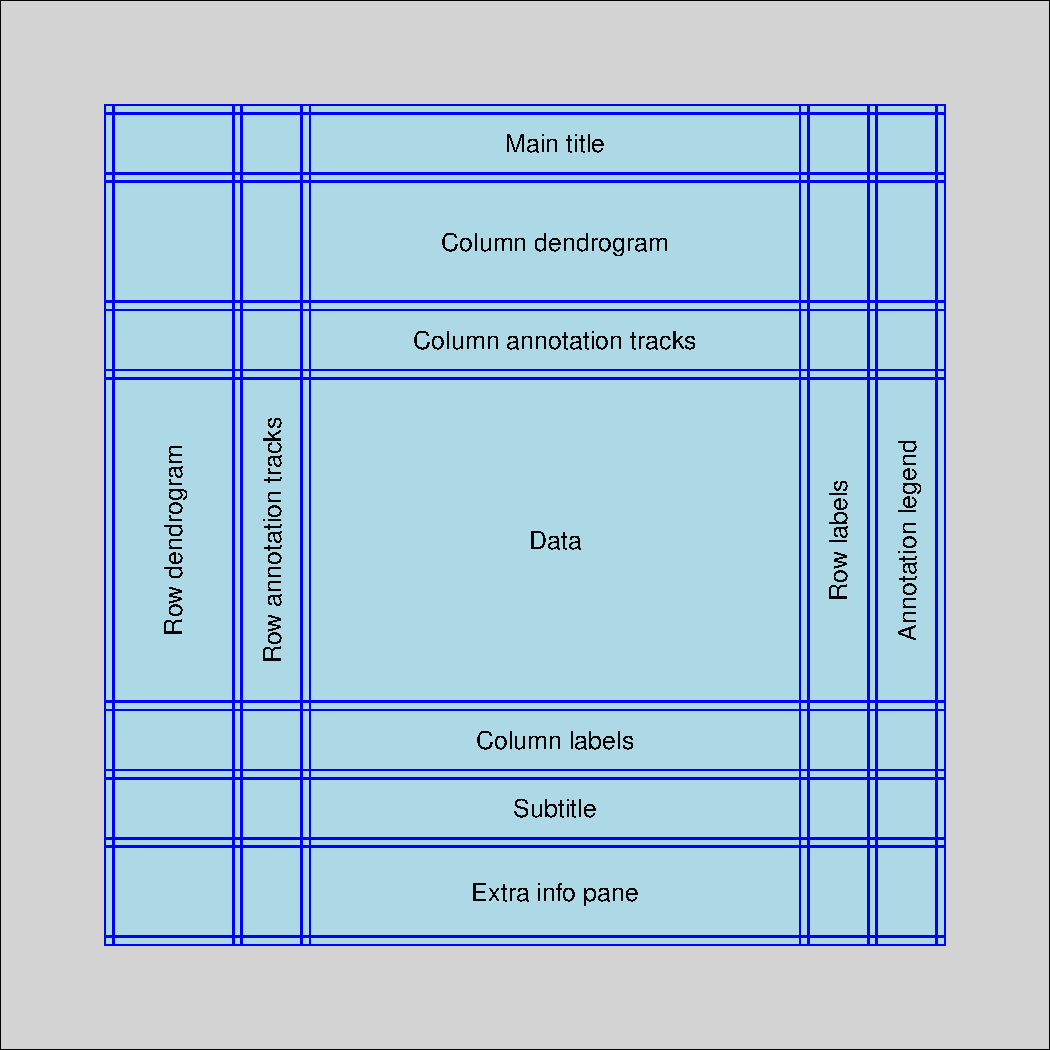
\includegraphics[width=.48\textwidth]{/home/renaud/Documents/projects/NMF/pkg/vignettes/figure/aheatmaps-layout1} 
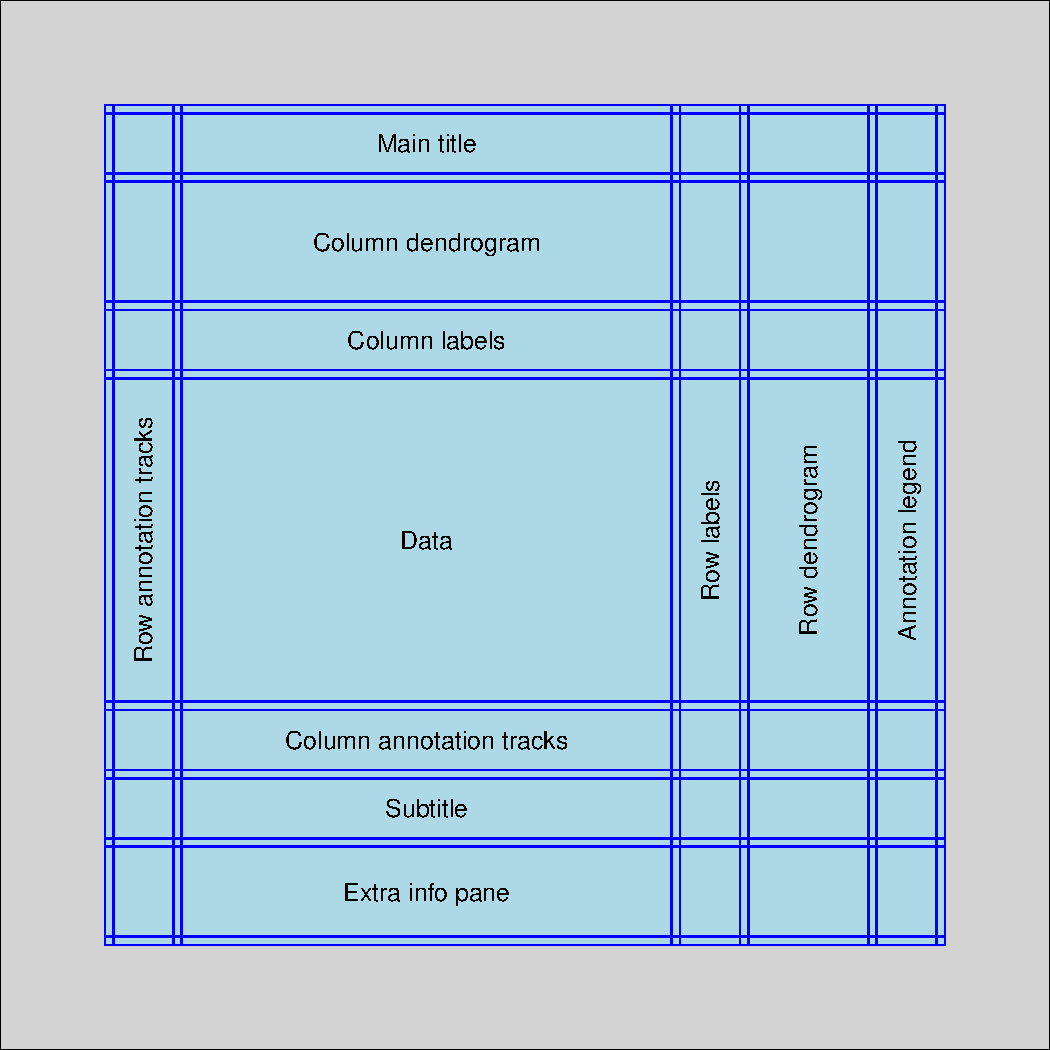
\includegraphics[width=.48\textwidth]{/home/renaud/Documents/projects/NMF/pkg/vignettes/figure/aheatmaps-layout2} 

\end{knitrout}
\caption{Grid layout diagram of annotated heatmaps: (left) default layout and
(right) an alternative layout, with separate specification for rows
and columns -- passed as a single string.}
\label{fig:layout}
\end{figure}

\section{Annotation tracks}

\section{Column/row ordering}

The rows and/or columns of heatmaps are generally ordered in a way that
highlight shared value patterns.
This ordering can be automatically computed from the data itself, using
hierarchical clustering algorithms, or forced to match known groups/order.
Arguments \code{Rowv}, \code{Colv}, as well as \code{distfun} and
\code{hclustfun} for automatic clustering, control how the ordering is
performed and displayed.
They accept the same values as the base function \code{aheatmap}, mimicking its
behaviour, but also supports other convenient ways of specifying ordering and
highlighting data patterns, some of which are illustrated in the rest of this
section.
We refer to the corresponding argument description on the man page
\code{?aheatmap} for a list of all supported values.

\subsection{Hierarchical clustering and dendrograms}
Dendrograms display result of applying a hierarchical clutering
algorithm to the rows or columns, typically using the base function \code{hclust}.

By default \code{aheatmap} performs hierarchical clustering and show the
associated dedrograms of both rows and columns, using the \code{"euclidean"}
distance and the linkage method \code{"complete"}.
However more custom clustering can also be specified:

\begin{knitrout}\small
\definecolor{shadecolor}{rgb}{0.969, 0.969, 0.969}\color{fgcolor}\begin{kframe}
\begin{alltt}
\hlcom{# default}
\hlkwd{aheatmap}\hlstd{(x)}
\hlcom{# use different clustering method for rows}
\hlkwd{aheatmap}\hlstd{(x,} \hlkwc{Rowv} \hlstd{=} \hlkwd{c}\hlstd{(}\hlstr{'manhattan'}\hlstd{,} \hlstr{'average'}\hlstd{),} \hlkwc{info} \hlstd{=} \hlnum{TRUE}\hlstd{)}
\hlcom{# use enternally computed clustering}
\hlstd{hc} \hlkwb{<-} \hlkwd{hclust}\hlstd{(}\hlkwd{dist}\hlstd{(x,} \hlkwc{method} \hlstd{=} \hlstr{'minkowski'}\hlstd{),} \hlkwc{method} \hlstd{=} \hlstr{'centroid'}\hlstd{)}
\hlkwd{aheatmap}\hlstd{(x,} \hlkwc{Rowv} \hlstd{= hc,} \hlkwc{info} \hlstd{=} \hlnum{TRUE}\hlstd{)}
\end{alltt}
\end{kframe}
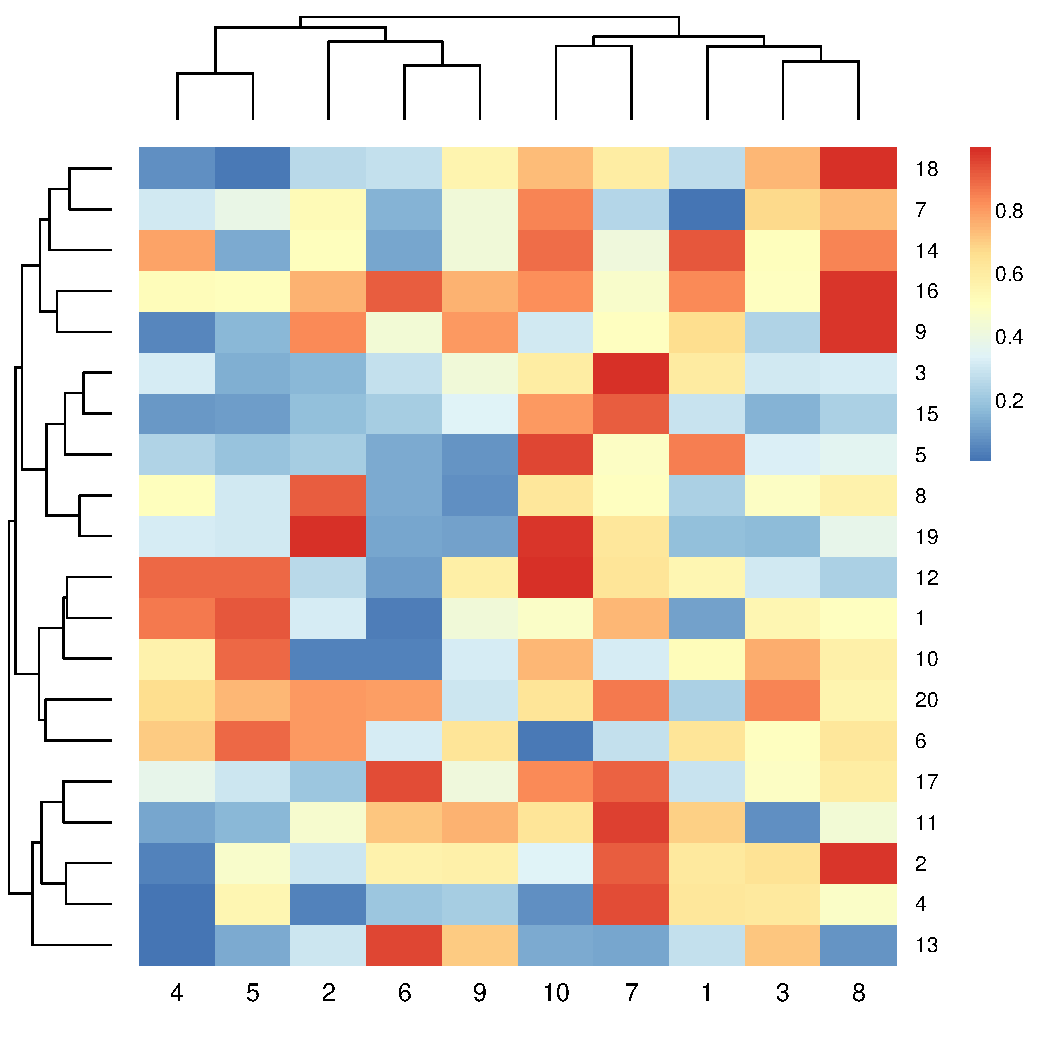
\includegraphics[width=0.33\textwidth]{/home/renaud/Documents/projects/NMF/pkg/vignettes/figure/aheatmaps-clustering1} 
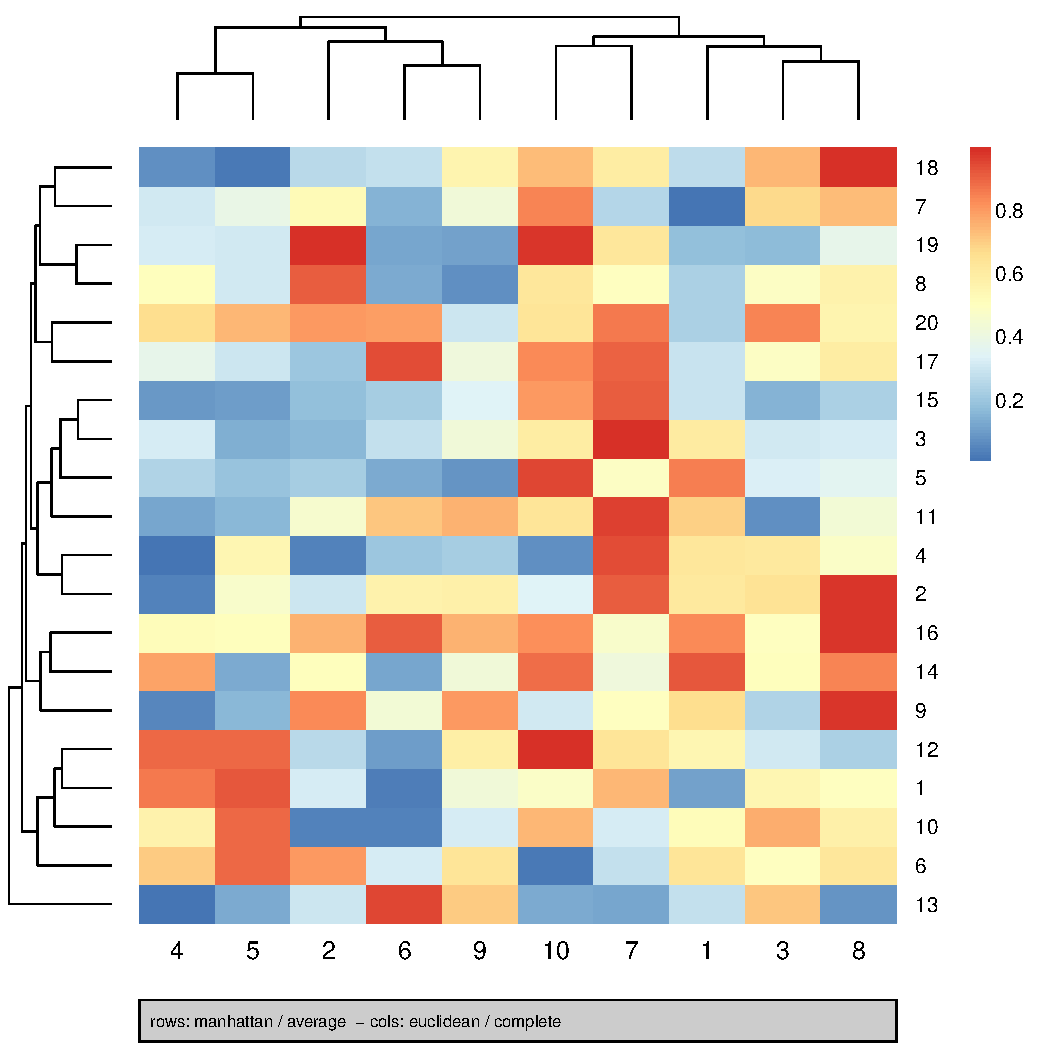
\includegraphics[width=0.33\textwidth]{/home/renaud/Documents/projects/NMF/pkg/vignettes/figure/aheatmaps-clustering2} 
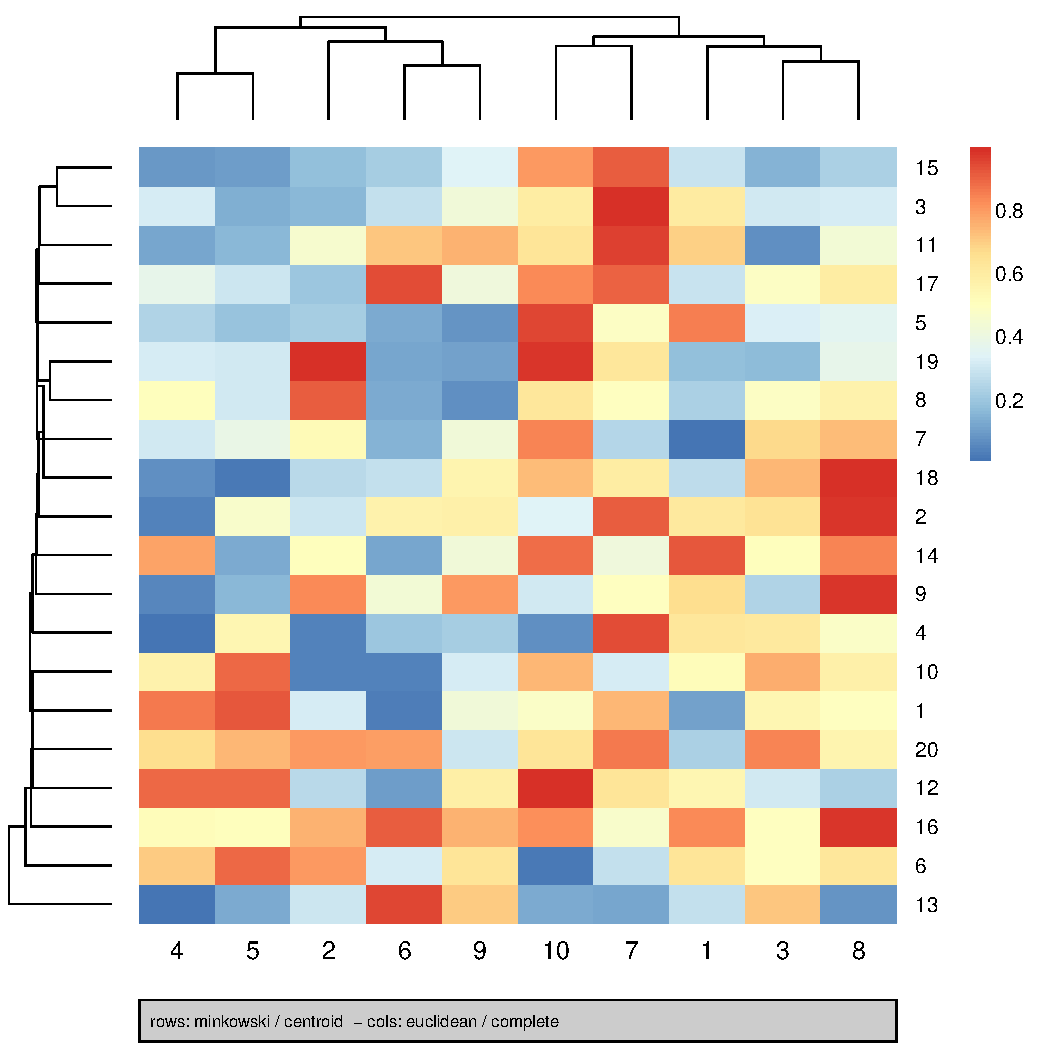
\includegraphics[width=0.33\textwidth]{/home/renaud/Documents/projects/NMF/pkg/vignettes/figure/aheatmaps-clustering3} 

\end{knitrout}

\subsubsection{Display}

\begin{knitrout}\small
\definecolor{shadecolor}{rgb}{0.969, 0.969, 0.969}\color{fgcolor}\begin{kframe}
\begin{alltt}
\hlcom{# cluster rows but do not show dendrogram}
\hlkwd{aheatmap}\hlstd{(x,} \hlkwc{Rowv} \hlstd{=} \hlnum{FALSE}\hlstd{)}
\hlcom{# cut column dendrogram into 3 clusters}
\hlkwd{aheatmap}\hlstd{(x,} \hlkwc{Rowv} \hlstd{=} \hlnum{FALSE}\hlstd{,} \hlkwc{Colv} \hlstd{=} \hlnum{3L}\hlstd{)}
\hlkwd{aheatmap}\hlstd{(x,} \hlkwc{Rowv} \hlstd{=} \hlnum{FALSE}\hlstd{,} \hlkwc{Colv} \hlstd{=} \hlopt{-}\hlnum{3L}\hlstd{)}
\end{alltt}
\end{kframe}
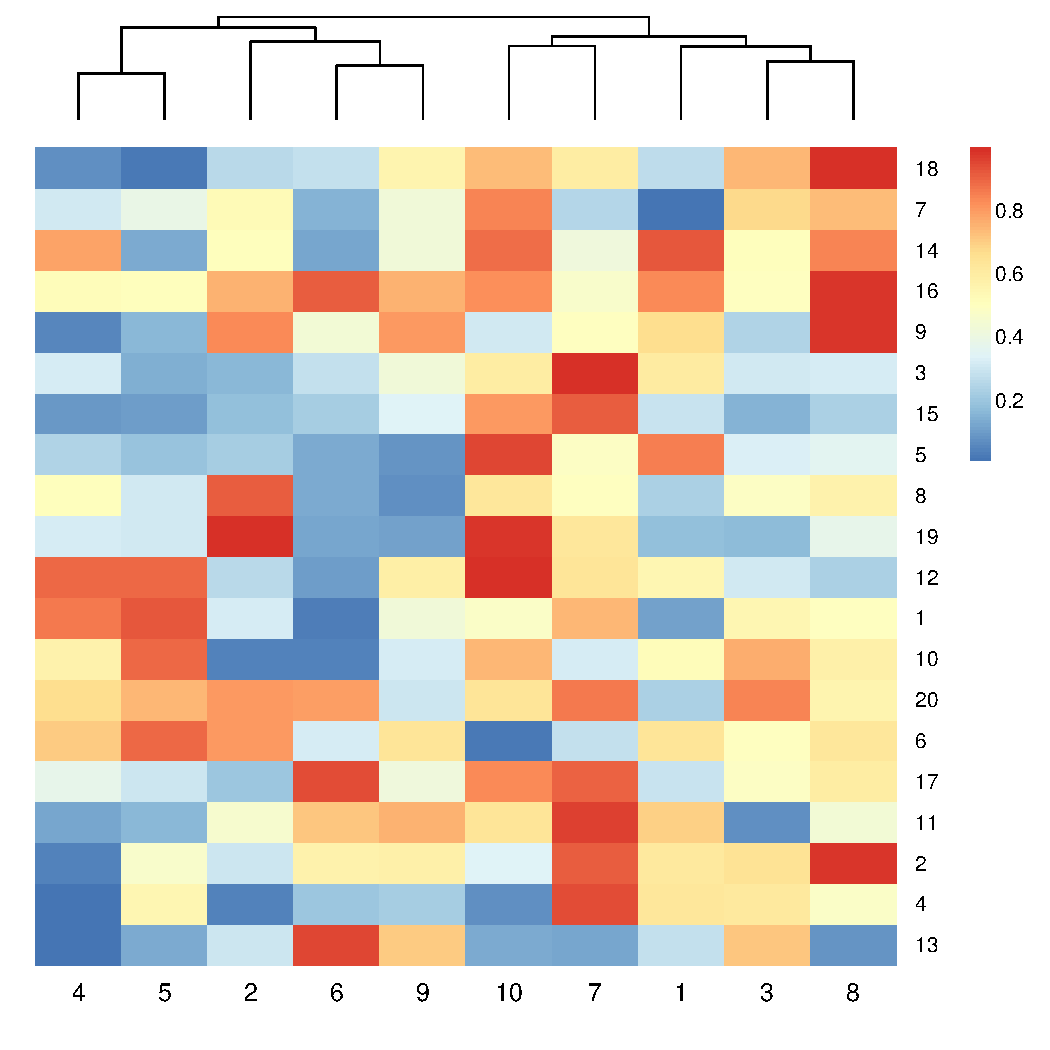
\includegraphics[width=0.33\textwidth]{/home/renaud/Documents/projects/NMF/pkg/vignettes/figure/aheatmaps-dendrogram1} 
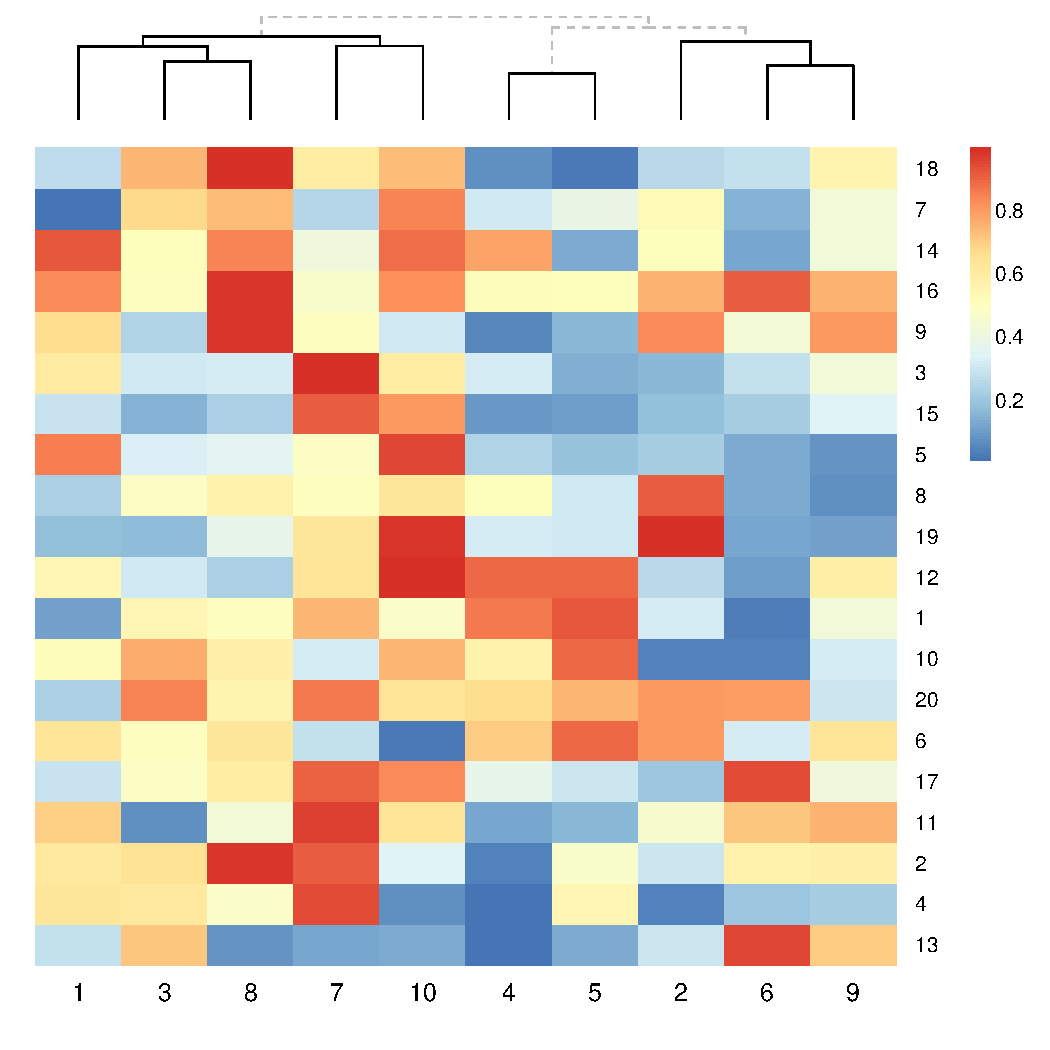
\includegraphics[width=0.33\textwidth]{/home/renaud/Documents/projects/NMF/pkg/vignettes/figure/aheatmaps-dendrogram2} 
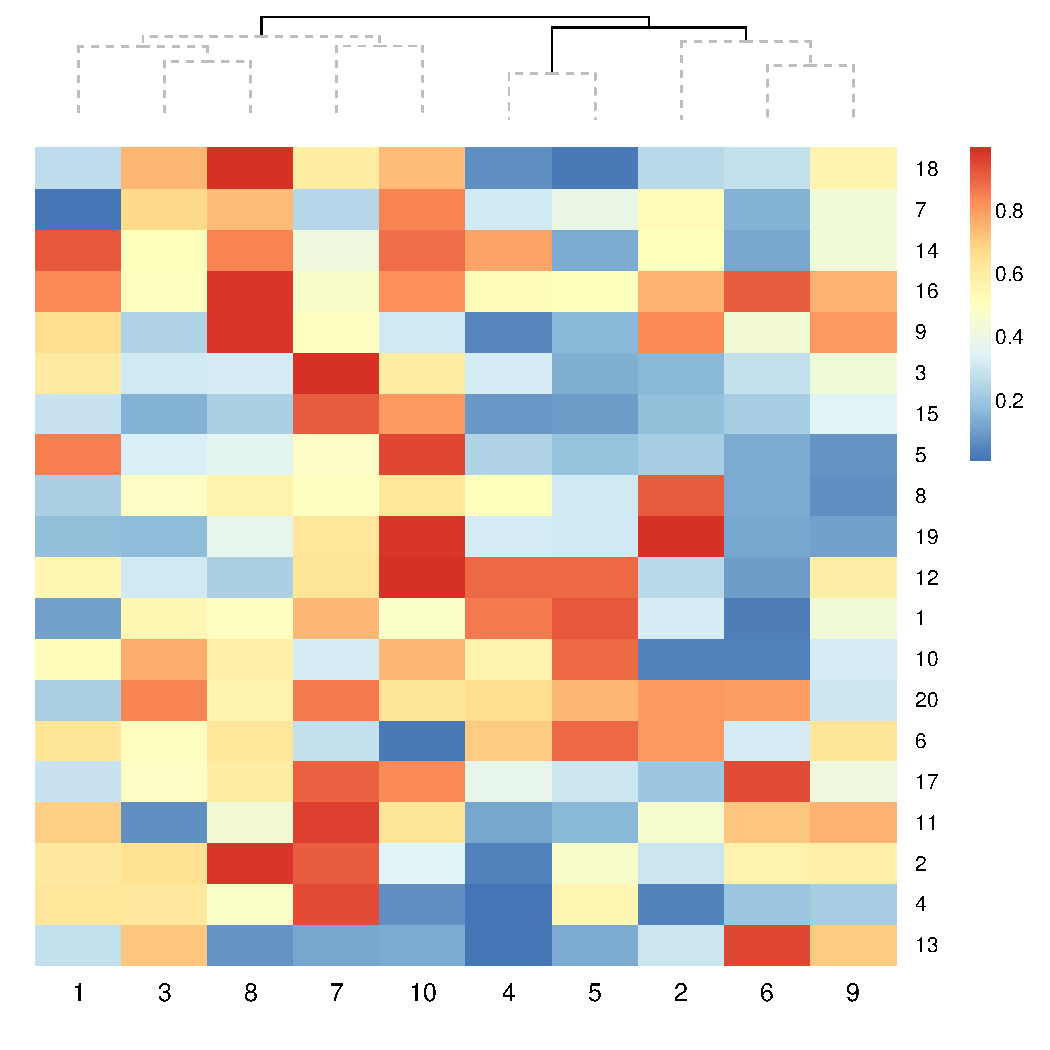
\includegraphics[width=0.33\textwidth]{/home/renaud/Documents/projects/NMF/pkg/vignettes/figure/aheatmaps-dendrogram3} 

\end{knitrout}

\code{aheatmap} also provides some convenient shortcuts to use the
\CRANpkg{dendextend} and produce enhanced cluster highlighting, with colors,
text and boxes:
\begin{knitrout}\small
\definecolor{shadecolor}{rgb}{0.969, 0.969, 0.969}\color{fgcolor}\begin{kframe}
\begin{alltt}
\hlcom{# cluster highlighting}
\hlkwd{aheatmap}\hlstd{(x,} \hlkwc{Rowv} \hlstd{=} \hlstr{"#4"}\hlstd{,} \hlkwc{Colv} \hlstd{=} \hlnum{FALSE}\hlstd{,} \hlkwc{main} \hlstd{=} \hlstr{"Colored clusters"}\hlstd{)}
\hlkwd{aheatmap}\hlstd{(x,} \hlkwc{Rowv} \hlstd{=} \hlstr{"#4|!"}\hlstd{,} \hlkwc{Colv} \hlstd{=} \hlnum{FALSE}\hlstd{,} \hlkwc{main} \hlstd{=} \hlstr{"Boxed clusters"}\hlstd{)}
\hlcom{# highlight cluster #2 only adding some red text}
\hlkwd{aheatmap}\hlstd{(x,} \hlkwc{Colv} \hlstd{=} \hlkwd{list}\hlstd{(}\hlstr{"#3@2"}\hlstd{,} \hlkwc{text_col} \hlstd{=} \hlstr{'red'}\hlstd{,} \hlkwc{text} \hlstd{=} \hlstr{'Cluster B'}\hlstd{),} \hlkwc{Rowv} \hlstd{=} \hlnum{FALSE}
            \hlstd{,} \hlkwc{main} \hlstd{=} \hlstr{"Partial highlithing"}\hlstd{)}
\end{alltt}
\end{kframe}
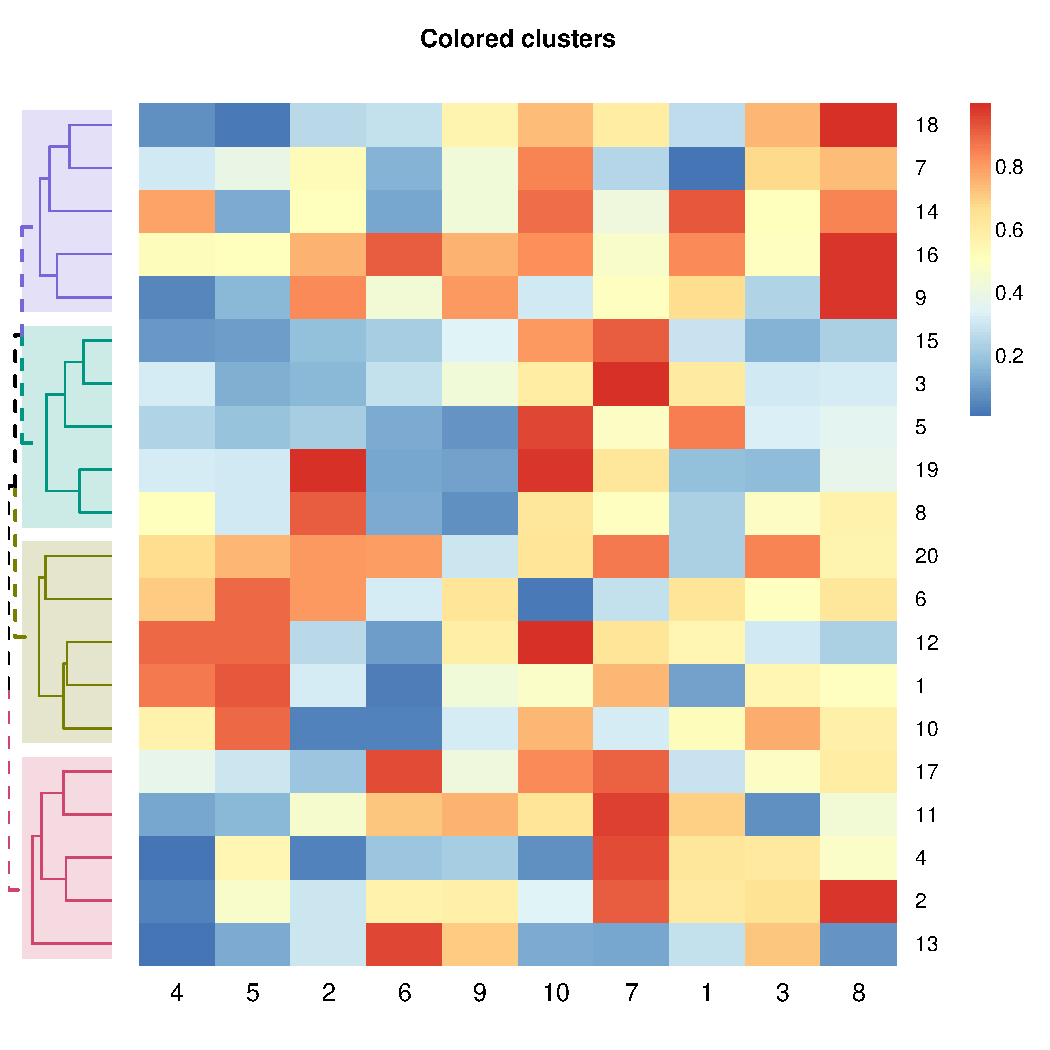
\includegraphics[width=0.33\textwidth]{/home/renaud/Documents/projects/NMF/pkg/vignettes/figure/aheatmaps-dendrogram_dendextend1} 
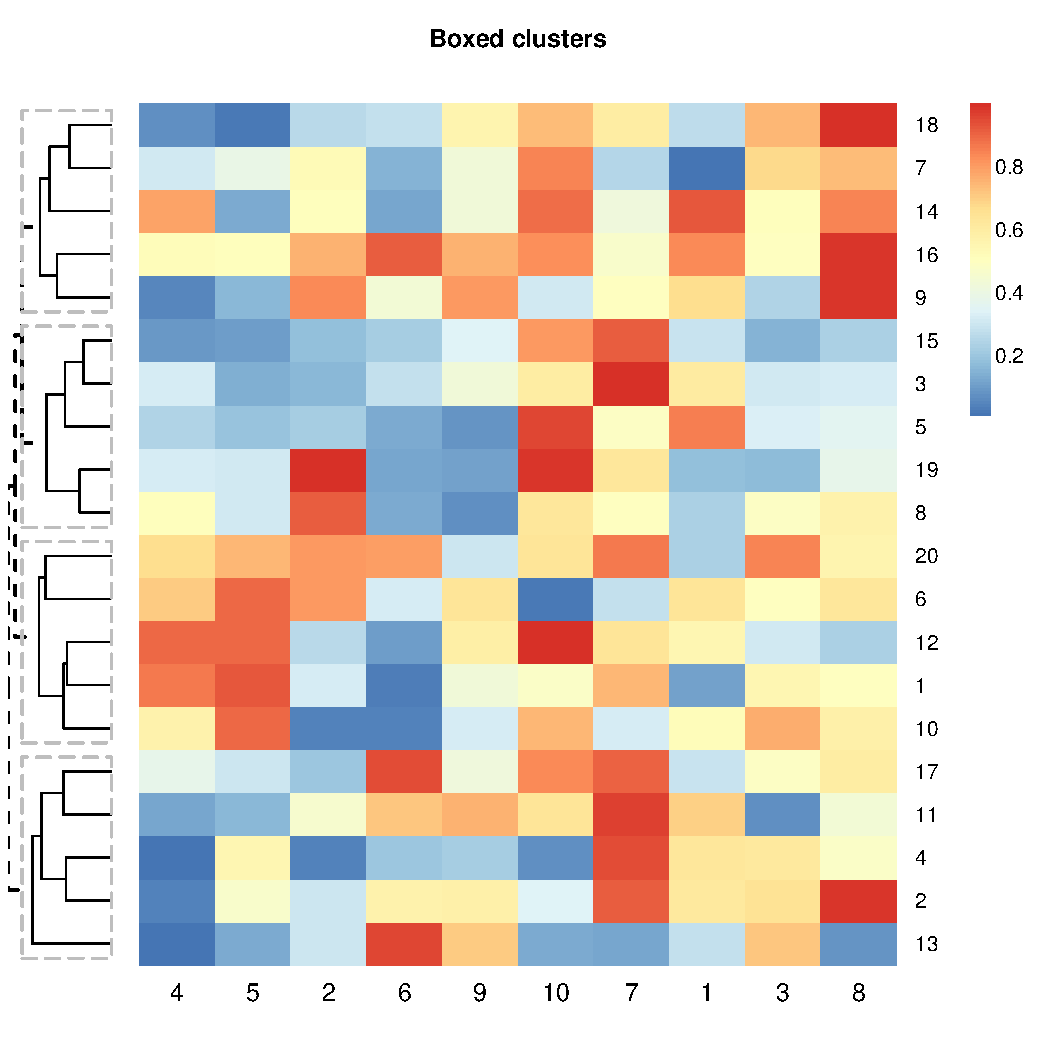
\includegraphics[width=0.33\textwidth]{/home/renaud/Documents/projects/NMF/pkg/vignettes/figure/aheatmaps-dendrogram_dendextend2} 
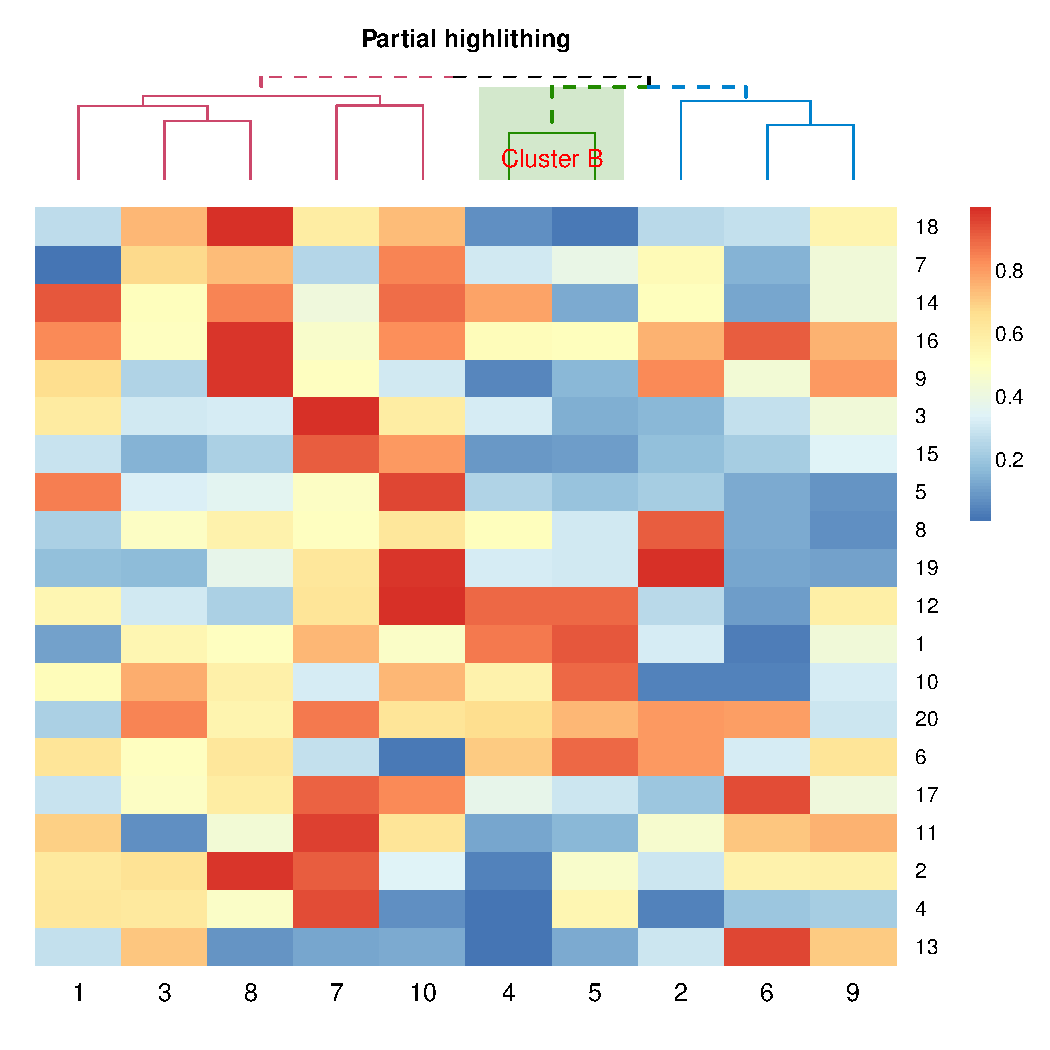
\includegraphics[width=0.33\textwidth]{/home/renaud/Documents/projects/NMF/pkg/vignettes/figure/aheatmaps-dendrogram_dendextend3} 

\end{knitrout}

A completely custom pre-formatted dendrogram can also be build and passed to
\code{Rowv} (or \code{Colv}), controlling both ordering and display.
For example, using the \pkgname{dendextend} package\footnote{Code borrowed
from
\url{http://cran.r-project.org/web/packages/dendextend/vignettes/introduction.html}},
one can format a dendrogram in a complex way and simply ``plug" it into the row
or column dendrogram panel:

\begin{adjustbox}{valign=t}
\begin{minipage}{.59\linewidth}
\begin{knitrout}\small
\definecolor{shadecolor}{rgb}{0.969, 0.969, 0.969}\color{fgcolor}\begin{kframe}
\begin{alltt}
\hlcom{# use pre-formatted dedrogram}
\hlkwd{library}\hlstd{(dendextend)}
\hlstd{hc} \hlkwb{<-} \hlkwd{hclust}\hlstd{(}\hlkwd{dist}\hlstd{(}\hlkwd{t}\hlstd{(x)))}
\hlstd{hc} \hlkwb{<-} \hlkwd{as.dendrogram}\hlstd{(hc)} \hlopt
        \hlkwd{set}\hlstd{(}\hlstr{"nodes_pch"}\hlstd{,} \hlkwd{c}\hlstd{(}\hlnum{19}\hlstd{,}\hlnum{1}\hlstd{,}\hlnum{4}\hlstd{))} \hlopt
        \hlkwd{set}\hlstd{(}\hlstr{"nodes_cex"}\hlstd{,} \hlkwd{c}\hlstd{(}\hlnum{2}\hlstd{,}\hlnum{1}\hlstd{,}\hlnum{2}\hlstd{))} \hlopt
        \hlkwd{set}\hlstd{(}\hlstr{"nodes_col"}\hlstd{,} \hlkwd{c}\hlstd{(}\hlnum{3}\hlstd{,}\hlnum{4}\hlstd{))}
\hlstd{hc} \hlkwb{<-} \hlstd{hc} \hlopt \hlkwd{set}\hlstd{(}\hlstr{"branches_lwd"}\hlstd{,} \hlkwd{c}\hlstd{(}\hlnum{4}\hlstd{,}\hlnum{1}\hlstd{))} \hlopt
           \hlkwd{set}\hlstd{(}\hlstr{"branches_lty"}\hlstd{,} \hlkwd{c}\hlstd{(}\hlnum{1}\hlstd{,}\hlnum{1}\hlstd{,}\hlnum{3}\hlstd{))} \hlopt
           \hlkwd{set}\hlstd{(}\hlstr{"branches_col"}\hlstd{,} \hlkwd{c}\hlstd{(}\hlnum{1}\hlstd{,}\hlnum{2}\hlstd{,}\hlnum{3}\hlstd{))}
\hlkwd{aheatmap}\hlstd{(x,} \hlkwc{Colv} \hlstd{= hc,} \hlkwc{Rowv} \hlstd{=} \hlnum{FALSE}
            \hlstd{,} \hlkwc{main} \hlstd{=} \hlstr{"Custom dendrogram"}\hlstd{)}
\end{alltt}
\end{kframe}
\end{knitrout}
\end{minipage}

\begin{minipage}{.4\linewidth}
\begin{knitrout}\small
\definecolor{shadecolor}{rgb}{0.969, 0.969, 0.969}\color{fgcolor}
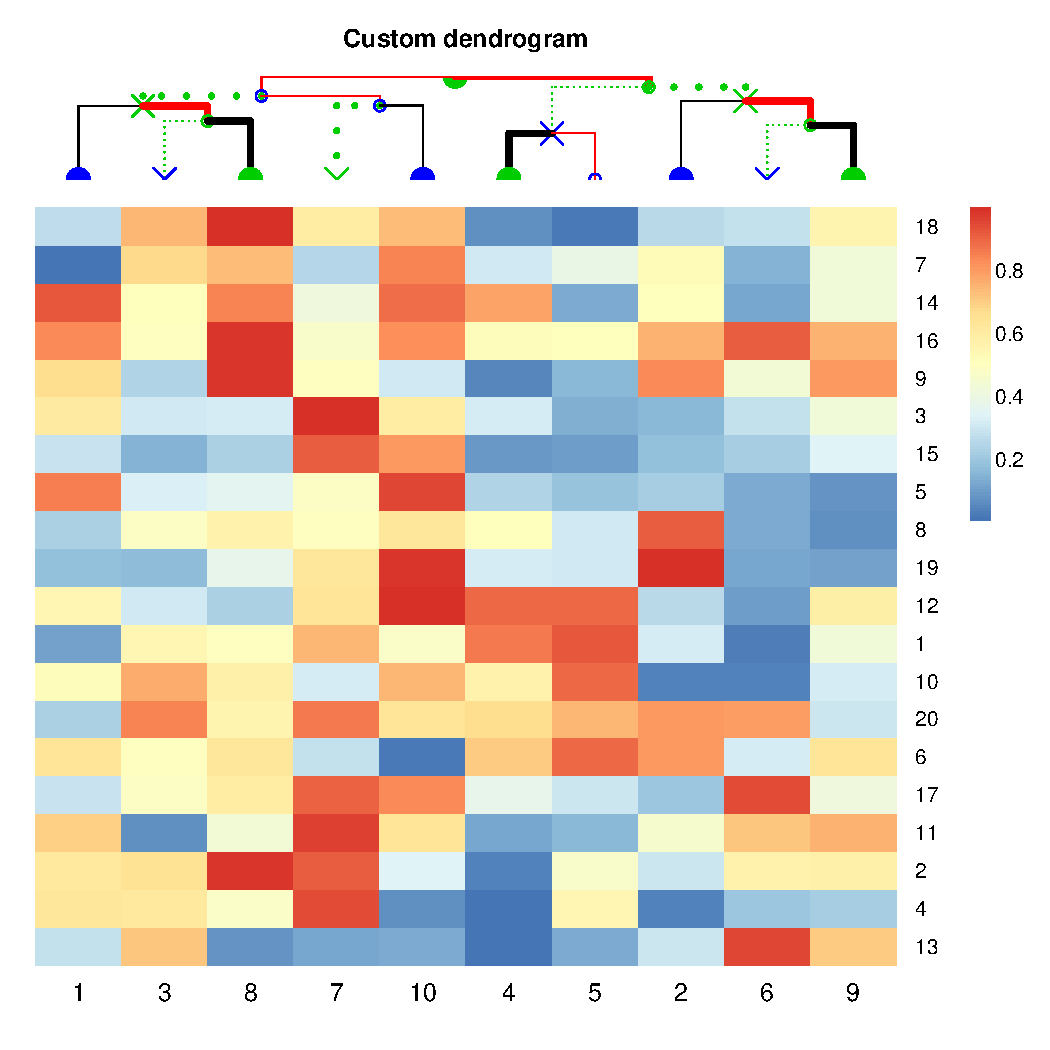
\includegraphics[width=\textwidth]{/home/renaud/Documents/projects/NMF/pkg/vignettes/figure/aheatmaps-dendrogram_custom_plot} 

\end{knitrout}
\end{minipage}
\end{adjustbox}


\subsection{Forced order}

Column and row order can also be forced to a given order by passing an
\textbf{integer} indexing vector or \code{NA} for keeping the original order.
It is important that the indexing vector is effectively an integer
vector, as passing a numeric vector would only provides weights used
when re-ordering the computed dendrogram.
When weights are used, the resulting dendrogram is essentially the same, with
branches (and leaves) ordered in different ways (see the two last heatmaps
below).

\begin{knitrout}\small
\definecolor{shadecolor}{rgb}{0.969, 0.969, 0.969}\color{fgcolor}\begin{kframe}
\begin{alltt}
\hlcom{# orignal order}
\hlkwd{aheatmap}\hlstd{(x,} \hlkwc{Rowv} \hlstd{=} \hlnum{NA}\hlstd{,} \hlkwc{Colv} \hlstd{=} \hlnum{NA}\hlstd{,} \hlkwc{main} \hlstd{=} \hlstr{'Original'}\hlstd{)}
\hlcom{# indexing vector}
\hlkwd{aheatmap}\hlstd{(x,} \hlkwc{Rowv} \hlstd{=} \hlnum{NA}\hlstd{,} \hlkwc{Colv} \hlstd{=} \hlkwd{seq}\hlstd{(}\hlkwd{ncol}\hlstd{(x),} \hlnum{1}\hlstd{),} \hlkwc{main} \hlstd{=} \hlstr{'Forced (inverse)'}\hlstd{)}
\hlcom{# not the same as numeric weight vector}
\hlkwd{aheatmap}\hlstd{(x,} \hlkwc{Rowv} \hlstd{=} \hlnum{NA}\hlstd{,} \hlkwc{Colv} \hlstd{=} \hlkwd{as.numeric}\hlstd{(}\hlkwd{seq}\hlstd{(}\hlkwd{nrow}\hlstd{(x),} \hlnum{1}\hlstd{)),} \hlkwc{main} \hlstd{=} \hlstr{'Values used as weights'}\hlstd{)}
\hlcom{# compare with no weights}
\hlkwd{aheatmap}\hlstd{(x,} \hlkwc{Rowv} \hlstd{=} \hlnum{NA}\hlstd{,} \hlkwc{main} \hlstd{=} \hlstr{'Default weighting'}\hlstd{)}
\end{alltt}
\end{kframe}
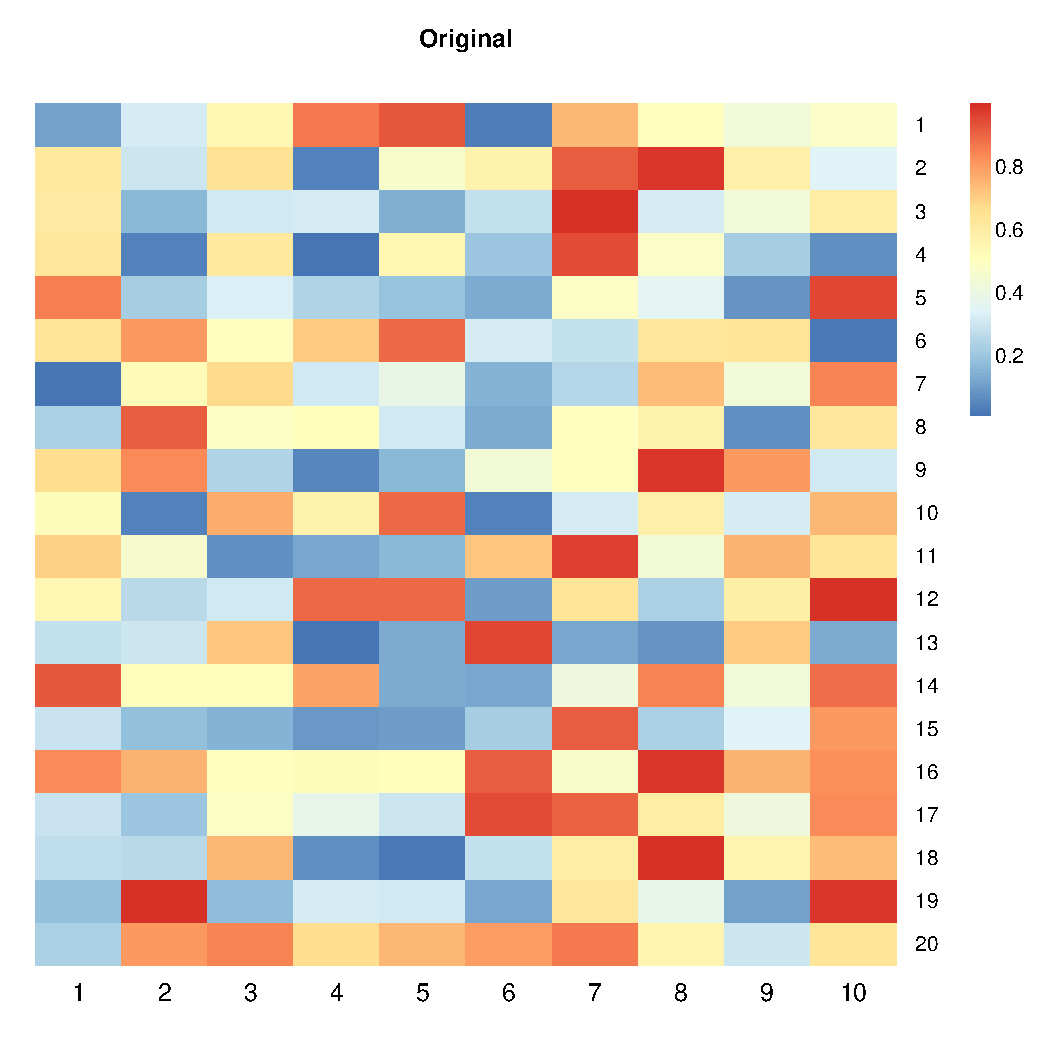
\includegraphics[width=.23\textwidth]{/home/renaud/Documents/projects/NMF/pkg/vignettes/figure/aheatmaps-dendrogram_custom_plot1} 
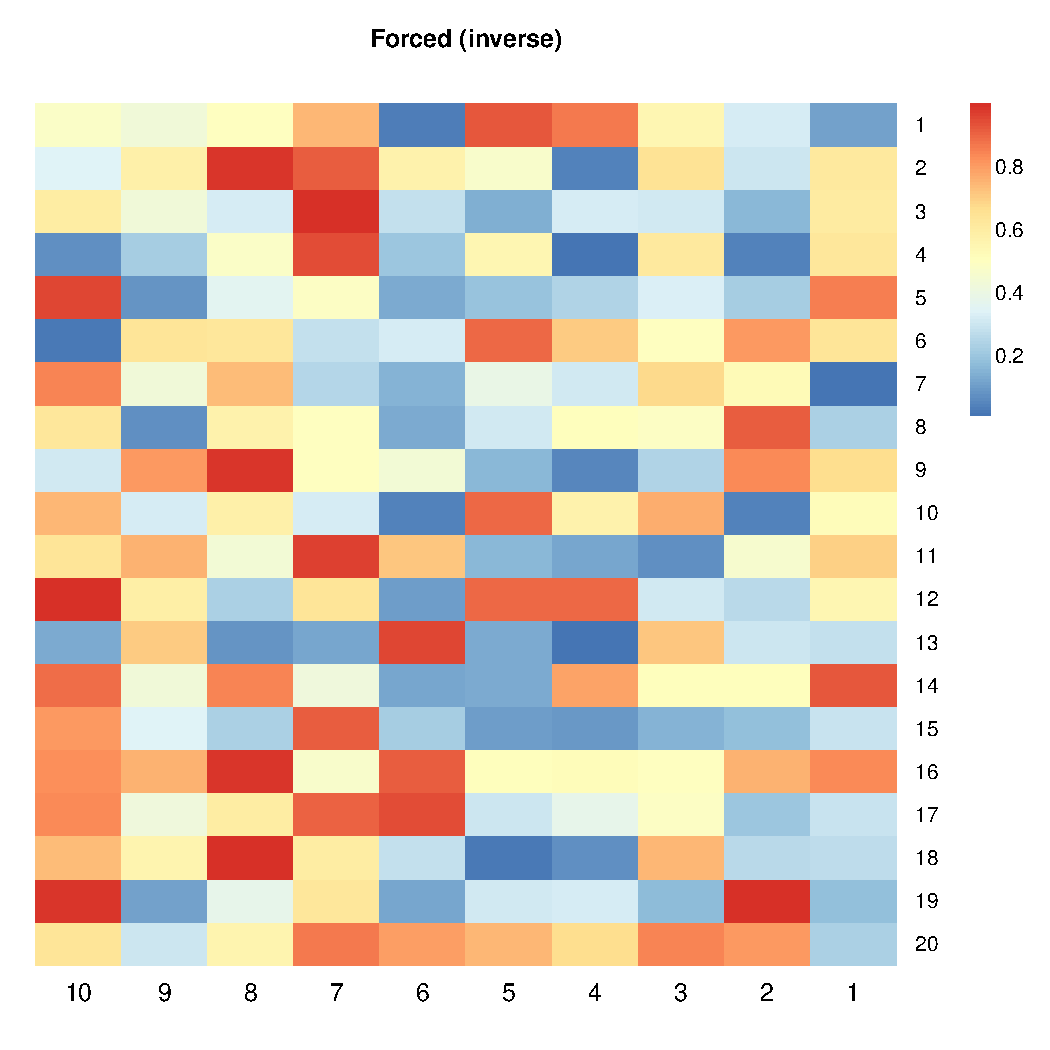
\includegraphics[width=.23\textwidth]{/home/renaud/Documents/projects/NMF/pkg/vignettes/figure/aheatmaps-dendrogram_custom_plot2} 
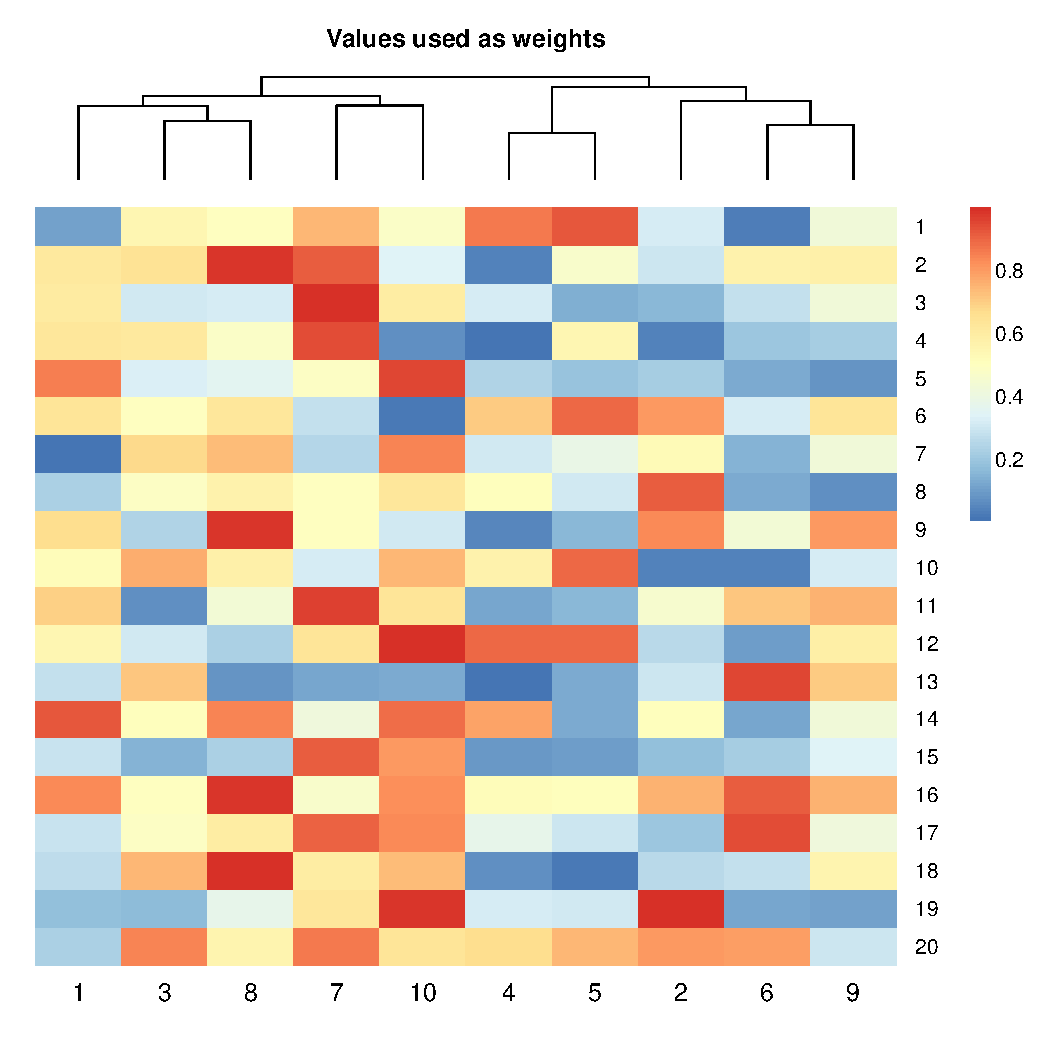
\includegraphics[width=.23\textwidth]{/home/renaud/Documents/projects/NMF/pkg/vignettes/figure/aheatmaps-dendrogram_custom_plot3} 
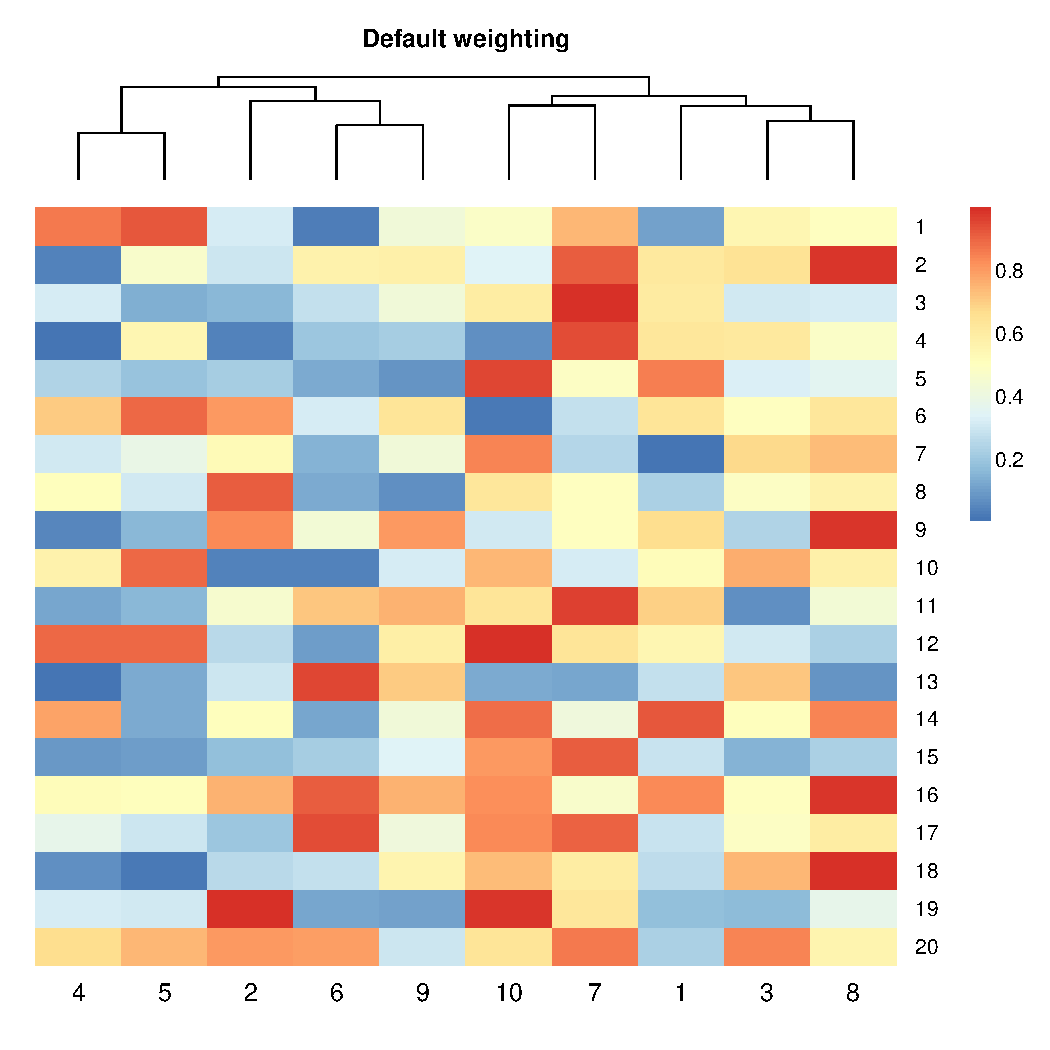
\includegraphics[width=.23\textwidth]{/home/renaud/Documents/projects/NMF/pkg/vignettes/figure/aheatmaps-dendrogram_custom_plot4} 

\end{knitrout}

\section{Colours}
\section{Labels}

\section{Legends}
Annotated heatmaps have two types of legends, one showing the colour-value scale
used to visualise the data matrix and another one for the annotation tracks.

\subsection{Colour scale}
The very principle of a heatmap is to bin data values into a certain number
of intervals (or breaks), associating each of these with a given colour.
The \emph{colour scale} is the legend that provides details about how to read
the resulting colour coded data matrix.
As such, it serves multiple purposes:
\begin{itemize}
  \item provide the mapping between colours and value intervals;
  \item show the actual range of displayed values;
  \item optionnaly show the overall distribution of values.
\end{itemize}

\subsubsection{Colours and breaks}

\subsubsection{Look and position}
As for other components in annotated heatmaps, the position of the
colour scale is controlled by the argument \code{layout}, which can also be used
to specify if the scale should expand over the full height/width or have a
limited fixed size.

By default the scale is placed on the top-right corner of the data matrix, with
a limited fixed size.
\Cref{fig:layout_scale} illustrates how to easily obtain some other commonly
used positions/look, through the use of special layout shortcuts.
More options are available, as detailed in the manual page for
\code{aheatmap\_layout}.

\begin{figure}[h!]
\begin{knitrout}\small
\definecolor{shadecolor}{rgb}{0.969, 0.969, 0.969}\color{fgcolor}\begin{kframe}
\begin{alltt}
\hlcom{# vertical on the right expanded over the full height}
\hlkwd{aheatmap}\hlstd{(x,} \hlkwc{layout} \hlstd{=} \hlstr{'*'}\hlstd{)}
\hlcom{# horizontal at the bottom-right corner}
\hlkwd{aheatmap}\hlstd{(x,} \hlkwc{layout} \hlstd{=} \hlstr{'_'}\hlstd{)}
\hlcom{# horizontal the bottom, expanded over the full width}
\hlkwd{aheatmap}\hlstd{(x,} \hlkwc{layout} \hlstd{=} \hlstr{'_*'}\hlstd{)}
\hlcom{# vertical on the left (when not using/showing row dendrogram)}
\hlkwd{aheatmap}\hlstd{(x,} \hlkwc{Rowv} \hlstd{=} \hlnum{NA}\hlstd{,} \hlkwc{layout} \hlstd{=} \hlstr{'^'}\hlstd{)}
\end{alltt}
\end{kframe}
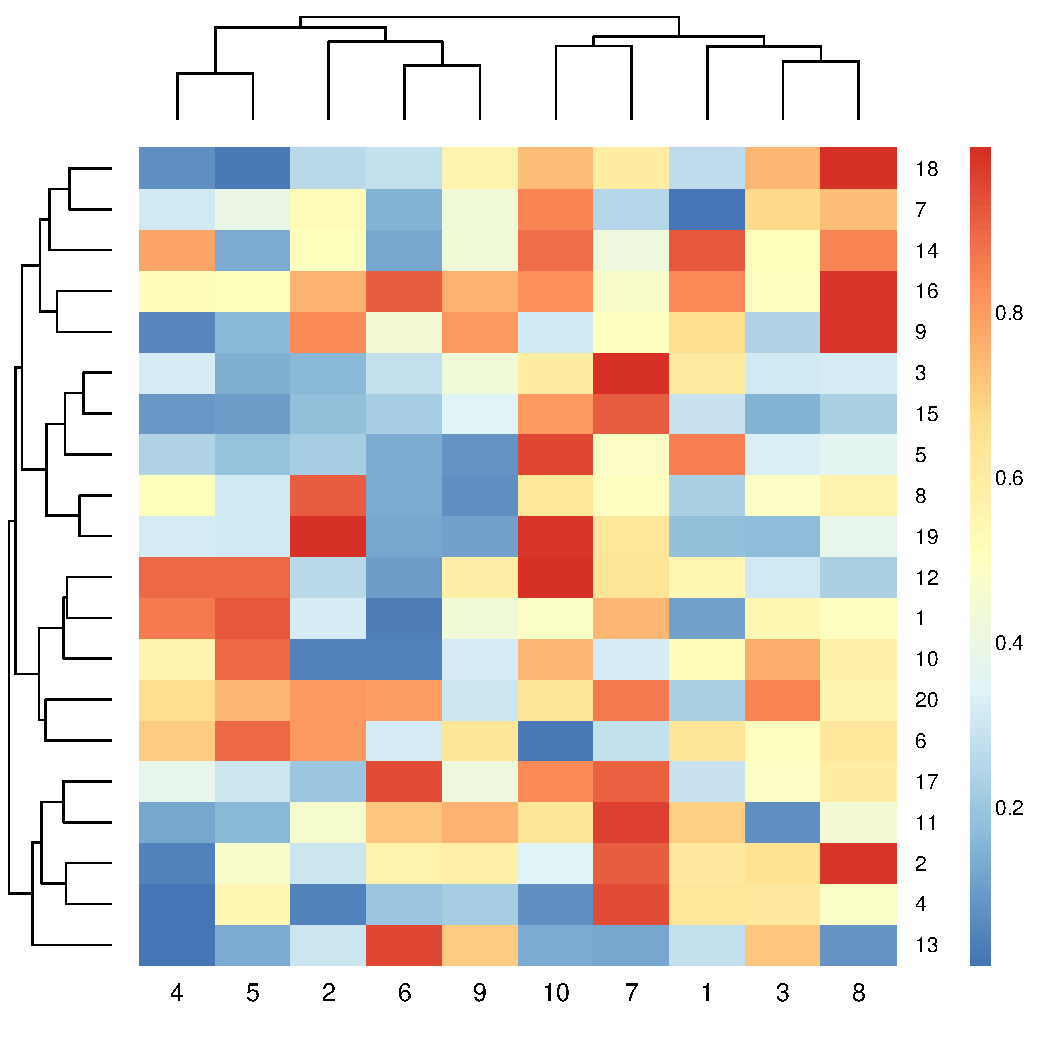
\includegraphics[width=0.23\textwidth]{/home/renaud/Documents/projects/NMF/pkg/vignettes/figure/aheatmaps-layout_scale1} 
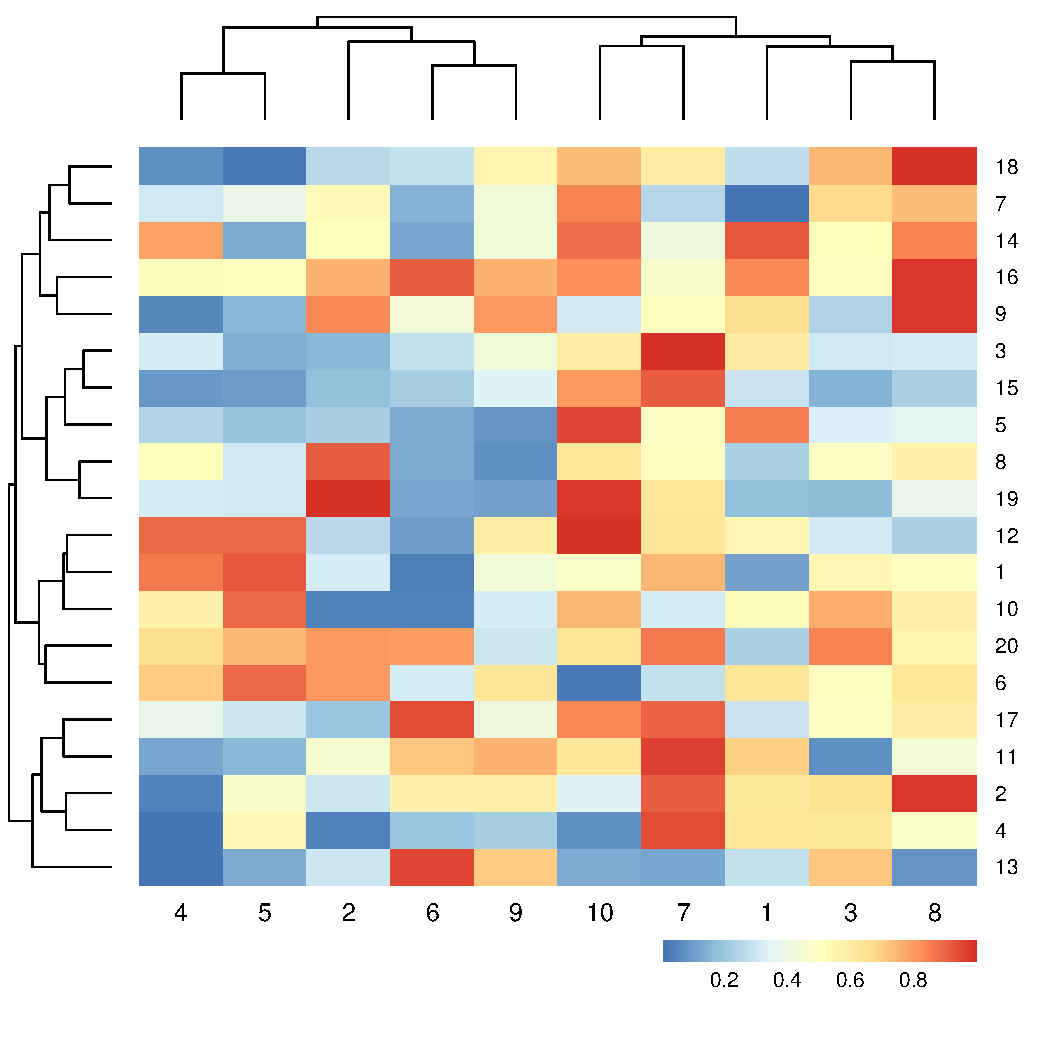
\includegraphics[width=0.23\textwidth]{/home/renaud/Documents/projects/NMF/pkg/vignettes/figure/aheatmaps-layout_scale2} 
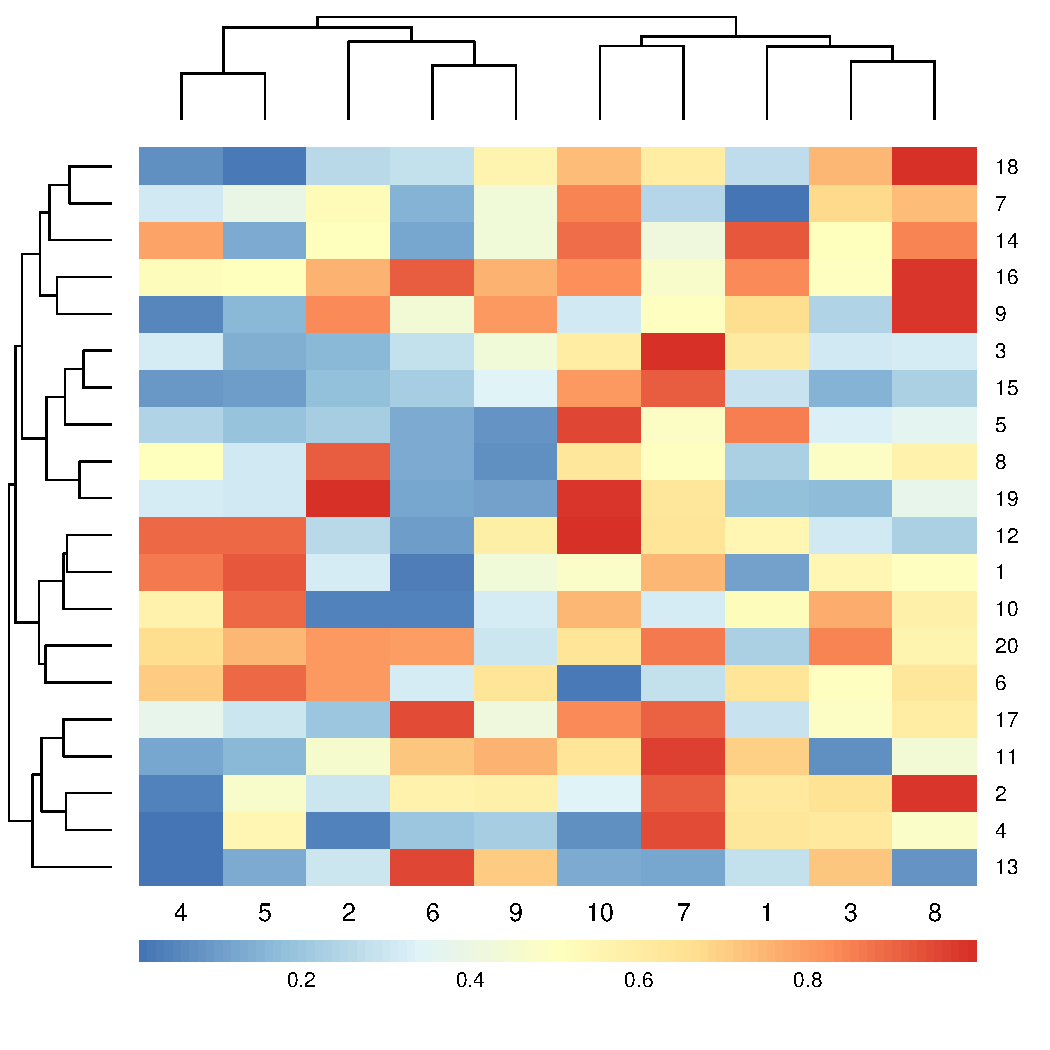
\includegraphics[width=0.23\textwidth]{/home/renaud/Documents/projects/NMF/pkg/vignettes/figure/aheatmaps-layout_scale3} 
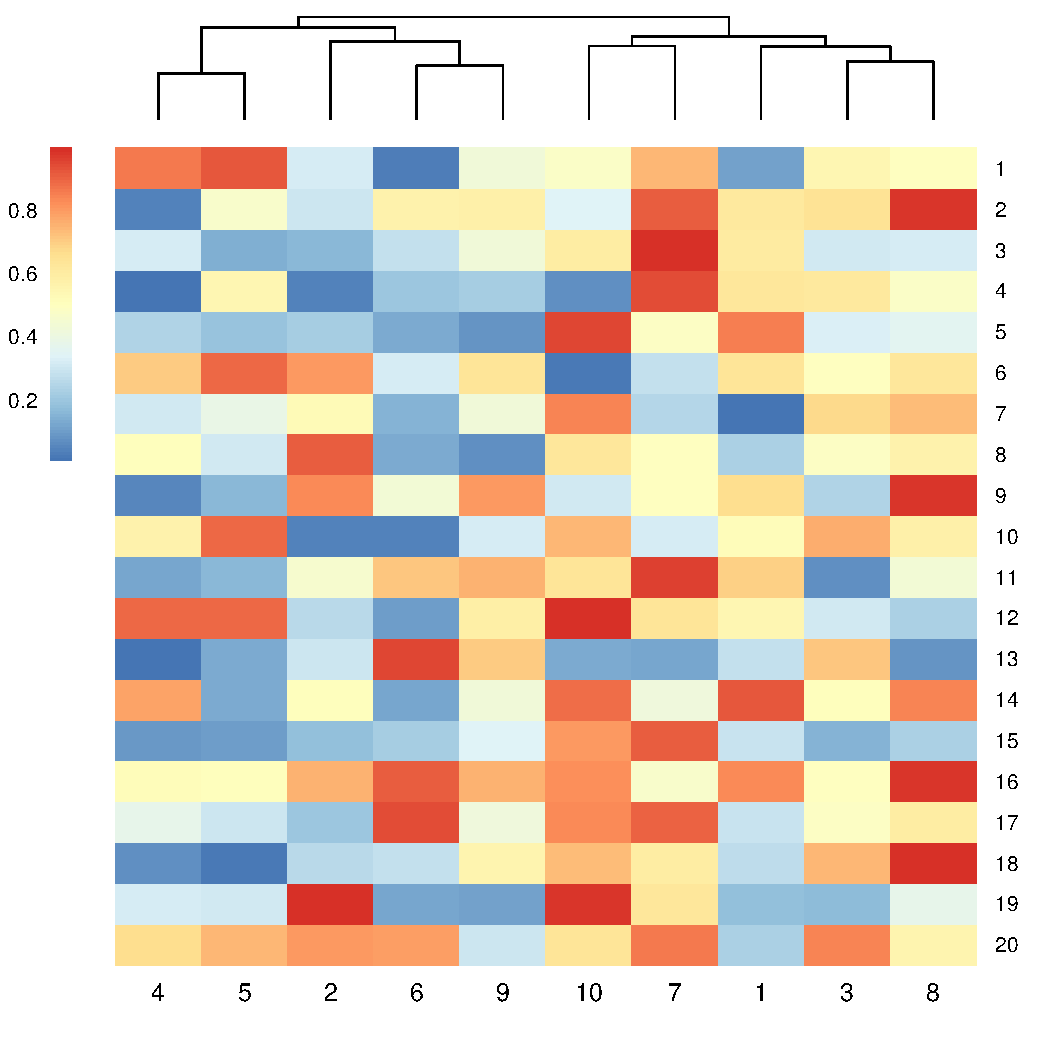
\includegraphics[width=0.23\textwidth]{/home/renaud/Documents/projects/NMF/pkg/vignettes/figure/aheatmaps-layout_scale4} 

\end{knitrout}
\caption{Colour scale alternative layouts: the scale can be placed in different
areas around the data matrix and expanded to full height/width.}
\label{fig:layout_scale}
\end{figure}


\subsection{Annotations}

\section{Session Info}
\begin{itemize}\raggedright
  \item R version 3.1.1 (2014-07-10), \verb|x86_64-pc-linux-gnu|
  \item Locale: \verb|LC_CTYPE=en_US.UTF-8|, \verb|LC_NUMERIC=C|, \verb|LC_TIME=en_ZA.UTF-8|, \verb|LC_COLLATE=en_US.UTF-8|, \verb|LC_MONETARY=en_ZA.UTF-8|, \verb|LC_MESSAGES=en_US.UTF-8|, \verb|LC_PAPER=en_ZA.UTF-8|, \verb|LC_NAME=C|, \verb|LC_ADDRESS=C|, \verb|LC_TELEPHONE=C|, \verb|LC_MEASUREMENT=en_ZA.UTF-8|, \verb|LC_IDENTIFICATION=C|
  \item Base packages: base, datasets, graphics, grDevices,
    methods, parallel, stats, utils
  \item Other packages: BH~1.54.0-3, bigmemory~4.4.6,
    bigmemory.sri~0.1.3, Biobase~2.24.0, BiocGenerics~0.10.0,
    cluster~1.15.2, colorspace~1.2-4, dendextend~0.17.1,
    knitr~1.6, NMF~0.21.3, pkgmaker~0.25.7, RColorBrewer~1.0-5,
    registry~0.2, rngtools~1.2.4, synchronicity~1.1.4
  \item Loaded via a namespace (and not attached):
    codetools~0.2-9, digest~0.6.4, doParallel~1.0.8,
    evaluate~0.5.5, foreach~1.4.2, formatR~1.0, ggplot2~1.0.0,
    grid~3.1.1, gridBase~0.4-7, gtable~0.1.2, highr~0.3,
    iterators~1.0.7, magrittr~1.0.1, MASS~7.3-34, munsell~0.4.2,
    plyr~1.8.1, proto~0.3-10, Rcpp~0.11.2, reshape2~1.4,
    scales~0.2.4, stringr~0.6.2, tools~3.1.1, whisker~0.3-2,
    xtable~1.7-3
\end{itemize}


\printbibliography[heading=bibintoc]

\end{document}
